
\section{Resumen}

El objetivo de este experimento es poder indetificar el coficiente de freflexion de una pastilla con seccion circular y de ancho presuntamente fijo.

Para ello se propone irradiar un area cuadrada delimitada por un "hierro" en el cual se pone una pantilla con un determinado indice de refracción, luego se define una grilla de posibles posiciones de donde se van a irradiar una señal $s(t)$ a dicha pastilla verticalmente, de forma de recuperar la señal original con una amplitud distinta y un corrimiento temporal debido al tiempo de vuelo de la señal (Ver Fig. \ref{fig:pastilla_transparente}).

Es de particular interes la fase de la señal recuperada dado que este es quien nos dará información sobre el material a analizar a traves de su indice de refracción.

Para ello se utiliza un \textit{chirp pulse} que tiene la particularidad de tenes una fase cuadratica tal que la relación frecuencia-tiempo es lineal, lo cual nos permite variar la frecuencia con el tiempo y de esa manera poder determinar frecuencias de interes facilmente.

\section{Física del problema}


\begin{figure}[H]
    \centering
        \resizebox{1.04\textwidth}{!}{%
            
\usetikzlibrary{decorations.pathmorphing,patterns,arrows.meta}

\begin{tikzpicture}[scale=0.9, >=stealth]

    % --- 1. CAPA DE FONDO: MARCO EN PERSPECTIVA ---
    \draw[gray!40, thin, fill=black!5] (0.8, 7.5) -- (4.2, 5.8) -- (4.2, -3.5) -- (0.8, -1.8) -- cycle;
    \draw[gray!40, dotted, thick] (0.8, 7.5) -- (0.8, -1.8);

    % --- 2. CAPA DE LA PASTILLA (Cuerpo y Relleno) ---

    \fill[blue!10, opacity=0.8]
        (1.5, 5.7) -- (2.7, 5.7)
        arc (90:-90:0.7cm and 2.7cm)
        -- (1.5, 0.3)
        arc (-90:90:0.7cm and 2.7cm)
        -- cycle;

    \draw[thick, blue!80!black]
        (2.7, 0.3) arc (-90:90:0.7cm and 2.7cm);

    \draw[thick, blue!80!black] (1.5, 5.7) -- (2.7, 5.7);
    \draw[thick, blue!80!black] (1.5, 0.3) -- (2.7, 0.3);

    \draw[
        thick,
        blue!80!black,
        fill=red!15,
        opacity=0.8,
        pattern=north east lines,
        pattern color=red!40
    ]
    (1.5, 3.0) ellipse[x radius=0.68cm, y radius=2.69cm];

    % --- 3. CAPA DE LÍNEAS INCIDENTES ---

    \foreach \y in {0.5,1.2,1.9,2.6,3.3,4.0,4.7,5.4}{
        \draw[thick, blue!80!black] (-5.5,\y) circle (0.12);
        \draw[thick, red!70!black] (-5.38,\y+0.03) -- (1.5,\y+0.03);
        \draw[thick, orange!90!black] (-5.38,\y-0.03) -- (2.7,\y-0.03);
    }

    % --- 4. CAPA DE ONDAS SUPERIORES ---

    \draw[dotted, ultra thick, black!60, samples=50, domain=-3.0:-1.2]
        plot (\x,{5.2 + 0.4*sin((\x+1.2)*180)});

    \draw[
        black!85,
        samples=100,
        domain=-1.2:1.5,
        arrows=-Latex,
        ultra thick
    ]
        plot (\x,{5.2 + 0.65*sin((\x+1.2)*130)});

    \draw[
        red!70,
        samples=100,
        domain=-5.6:1.4,
        arrows=Stealth-,
        ultra thick
    ]
        plot (\x,{5.2 + 0.55*sin((\x+1.8)*160 + 45)});

    \draw[
        thick,
        dash dot,
        samples=80,
        domain=2.7:-0.7,
        arrows=-Latex,
        densely dotted,
        orange!71
    ]
        plot (\x,{5.2 + 0.30*sin((\x+1.0)*500 - 30)});

    \draw[
        line width=1.2pt,
        blue,
        decorate,
        decoration={
            snake,
            segment length=7pt,
            amplitude=3.5pt
        },
        ->,
        densely dotted,
        /pgf/decoration/segment length=14.2pt,
        /pgf/decoration/amplitude=7.4pt
    ]
        (1.5,5.2) -- (2.8,5.2);

    % --- 5. CORTES Y COTAS DE MEDIDA ---

    \draw[dotted, thick] (1.5,5.7) -- (1.5,6.8);
    \draw[dotted, thick] (2.7,5.7) -- (2.7,6.8);

    \draw[<->, thick]
        (1.5,6.6) -- (2.7,6.6)
        node[midway,above]
        {$\Delta \tau \propto \Delta f$};

    \draw[dotted, thick] (1.5,0.3) -- (1.5,-2.4);
    \draw[dotted, thick] (2.7,0.3) -- (2.7,-2.4);

    % --- 6. GRÁFICA INFERIOR ---

    \draw[->, thick]
        (-5.0,-2.5) -- (4.0,-2.5)
        node[right] {$f[Hz]$};

    \draw[->, thick]
        (-4.6,-3.0) -- (-4.6,-0.3)
        node[above] {$|A|[\text{dB}]$};

    \draw[thick]
        (1.5,-2.4) -- (1.5,-2.6)
        node[below=2pt,blue!80!black] {\large $f_1$};

    \draw[thick]
        (2.7,-2.4) -- (2.7,-2.6)
        node[below=2pt,blue!80!black] {\large $f_2$};

    \draw[dotted, thin, black!70]
        (0.5,-2.1) -- (2.5,-1.0);

    \draw[line width=1.5pt, blue!80!black, smooth]
        (-4.5,-2.1)
        .. controls (-4.0,-2.1) and (-3.8,-1.8) .. (-3.5,-1.8)
        .. controls (-3.3,-2.2) and (-3.1,-1.5) .. (-2.8,-1.5)
        .. controls (-2.6,-2.2) and (-2.3,-1.8) .. (-2.0,-1.8)
        .. controls (-1.5,-2.2) and (-1.0,-2.2) .. (-0.44,-2.07)
        .. controls (0.8,-1.78) and (1.41,-1.11) .. (1.5,-0.12)
        .. controls (1.78,-1.68) and (1.87,-1.56) .. (2.16,-1.33)
        .. controls (2.5,-1.8) and (2.7,-0.4) .. (2.79,-1.19)
        .. controls (3.0,-1.8) and (3.3,-1.5) .. (3.8,-1.8);

\end{tikzpicture}

%
        }
        \caption{Representación en perspectiva del paso de ondas senoidales a través del volumen de la pastilla, con transparencia.}
    \label{fig:pastilla_transparente}
\end{figure}


\begin{figure}[H]
    \centering
    \resizebox{1.04\textwidth}{!}{%
        \begin{tikzpicture}[scale=1.2, >=stealth]
    % Ejes coordinados
    \draw[->, thick] (-0.3,0) -- (5,0) node[below left] {$t$};
    \draw[->, thick] (0,-0.3) -- (0,3.5);

    % Marcas y etiquetas en los ejes
    \draw[thick] (-0.1,1) -- (0.1,1) node[left, at start] {$f_0$};
    \draw[thick] (-0.1,3) -- (0.1,3) node[left=1pt, at start] {$f_0 + \beta$};
    \draw[thick] (2.2,-0.1) -- (2.2,0.1) node[below=1pt, at start] {$\tau$};

    % Líneas punteadas de proyección
    \draw[dotted, thick] (0,3) -- (2.2,3);
    \draw[dotted, thick] (2.2,0) -- (2.2,3);

    % Recta azul
    \draw[line width=1.2pt, blue!70!black] (0,1) -- (2.2,3);
\end{tikzpicture}
%
    }
    \caption{Relacion fase-frecuencia con tiempo de rampa $\tau$.}
    \label{fig:chirp_fig}
\end{figure}
Se define el \textit{pulso chirp} $s(t)$, cuya fase $\varphi(t)$ es una función dependiente del tiempo.

Lo interesante de esta fase es que, al derivarla, se observa una relación lineal entre la frecuencia instantánea y el tiempo:

\begin{equation}
    f_i(t) = f_0 + \frac{\beta}{\tau} t \quad \text{para } 0 < t < \tau
\end{equation}

donde $f_0$ y $\frac{\beta}{\tau}$ son constantes positivas, tal que.
\begin{itemize}
    \item $\beta$ es el ancho de banda.
    \item $f_0$ frecuencia de portadora.
    \item $\tau$ tiempo de rampa.
    \item $\frac{\beta}{\tau}$ \textit{chirp rate} (tasa de barrido)

\end{itemize}

Para hallar la expresión de la fase, se plantea la relación entre la frecuencia instantánea y la fase:

\begin{equation}
    f_i(t) = \frac{1}{2\pi} \frac{\partial \varphi(t)}{\partial t}
\end{equation}

Para el dominio temporal $t \in [0, \tau]$, integramos la frecuencia instantánea respecto al tiempo:

\begin{equation}
    \begin{aligned}
        \varphi(t) &= \int 2\pi f_i(t) \, dt \\
        \varphi(t) &= \int 2\pi \left[ f_0 + \frac{\beta}{\tau} t \right] dt \\
        \varphi(t) &= \frac{\pi\beta}{\tau} t^{2} + 2\pi f_0 t + C
    \end{aligned}
\end{equation}


Por lo tanto, la fase que define al \textit{chirp} es $\varphi(t) = \frac{\pi\beta}{\tau} t^{2} + 2\pi f_0 t + C$, por lo que el \textit{pulso chirp} resulta:

\begin{equation}
    \begin{aligned}
        s(t) &= a_0 e^{j\varphi(t)} \\
        &= a_0 e^{j \left( \frac{\pi\beta}{\tau} t^{2} + 2\pi f_0 t + C \right)} \\
        &= \overbrace{a_0 e^{jC}}^{a_1} e^{j \left( \frac{\pi\beta}{\tau} t^{2} + 2\pi f_0 t \right)} \\
        &= a_1 e^{j \left( \frac{\pi\beta}{\tau} t^{2} + 2\pi f_0 t \right)}
    \end{aligned}
\end{equation}

La señal recibida es proporcional a la señal transmitida $s(t)$. Dado que la onda debe recorrer una distancia $d$ de ida y vuelta hacia el objeto de interés, el receptor captura una réplica escalada y retrasada temporalmente $k s(t - t_0)$. Además, esta señal se ve afectada por ruido de diversas fuentes (como el ruido térmico del ADC), el cual se modela mediante el término $\epsilon(t)$.

Finalmente, la señal recibida se expresa como:

\begin{equation}
    \Gamma(t) = k s(t - t_0) + \epsilon(t) \quad \text{donde } t_0 = \frac{2d}{c} \quad \text{y } \epsilon(t) \text{ es el ruido.}
\end{equation}

En donde se propone la siguiente señal demoduladora para recuperar la señal.

\begin{equation}
    s_{dem} = e^{-j \left( \frac{\pi\beta}{\tau} t^{2} + 2\pi f_0 t \right)}
\end{equation}

de esta manera las frecuencias que obtenemos nos quedan constantes.

\begin{equation}
    \begin{aligned}
        s_{rec} &= ks(t-t_0).s_{dem}\\
        &= k e^{j \left( \frac{\pi\beta}{\tau} (t-t_0)^{2} + 2\pi f_0 (t-t_0) \right)} e^{-j \left( \frac{\pi\beta}{\tau} t^{2} + 2\pi f_0 t \right)}\\
        &= k e^{j \left( \frac{\pi\beta}{\tau} [t^{2}+t_0^{2} -2tt_0] + 2\pi f_0 (t-t_0) \right)} e^{-j \left( \frac{\pi\beta}{\tau} t^{2} + 2\pi f_0 t \right)}\\
         &= k e^{j \left( \frac{\pi\beta}{\tau} [t_0^{2} -2tt_0] - 2\pi f_0 t_0 \right)}\\
         &= k e^{j \left( \frac{\pi\beta}{\tau} t_0^{2} - 2\pi f_0 t_0 \right)} \underbrace{e^{j\frac{\pi \beta}{\tau}2t_0 t}}_{sinoide}
    \end{aligned}
\end{equation}

Entonces, si miro la parte real de señal recuperada (demodulada) $s_{rec}$ es una senoide ponderada por una aplitud dependiente de la amplitud inicial se la señal original y $k$ siendo este el factor de  escalamiento de la señal reflejada.

\section{Obtención de frecuencias de interés}

Los datos son obtenidos mediante un \textbf{ADC} el cual devuelve un array con los valores en fase y cuadratura $I$, $Q$ consecutivamente en un solo canal.

%\begin{equation}
%\text{adc\_signal} = \left[ I_0,\, Q_0,\, I_1,\, Q_1,\, \ldots,\, I_n,\, Q_n \right]
%\end{equation}


\begin{figure}[H]
    \centering
    \resizebox{1.0\textwidth}{!}{%
        \begin{tikzpicture}[
    font=\small,
    >=stealth,
    block/.style={
        draw, 
        rounded corners=8pt, 
        minimum width=1.8cm, 
        minimum height=1.6cm, 
        align=center, 
        thick
    },
    adc/.style={
        draw, 
        signal, 
        signal to=right, 
        thick, 
        minimum height=0.9cm, 
        inner sep=4pt
    },
    subblock/.style={
        draw, 
        rounded corners=5pt, 
        minimum width=1.4cm, 
        minimum height=0.6cm, 
        align=center, 
        thick,
        font=\small
    }
]

    % ==========================================
    % FILA SUPERIOR: Procesamiento Inicial I/Q
    % ==========================================
    \node[adc] (adc) {ADC};
    \node[right=0.2cm of adc, draw, thick, inner sep=0pt] (stream) {%
        \begin{tabular}{|c|c|c|c|c@{}c@{}}
            $I_0$ & $Q_0$ & $I_1$ & $Q_2$ & \dots & \hspace{0.2cm}
        \end{tabular}%
    };
    \node[block, right=0.4cm of stream] (dc) {
        $I \leftarrow I - \langle I \rangle$ \\[0.2cm]
        $Q \leftarrow Q - \langle Q \rangle$
    };
    \node[block, right=0.5cm of dc] (win) {
        $I \leftarrow I \cdot W$ \\[0.2cm]
        $Q \leftarrow Q \cdot W$
    };
    \node[block, right=0.5cm of win] (fft1) {
        {\Large $\mathcal{F}[\cdot]$}
    };
    \node[subblock, right=0.8cm of fft1.south east, anchor=south west, yshift=0.40cm] (delay1) {delay};
    \node[subblock, below=0.12cm of delay1] (offset1) {offset};
    \node[block, right=1.2cm of delay1.east |- fft1, minimum height=1.8cm] (ijq) {
        {\Large $\mathcal{I} + j\mathcal{Q}$}
    };
    \draw[thick] (adc) -- (stream);
    \draw[thick] (stream.east) -- (dc);
    \draw[thick] ($(dc.east)+(0,0.3)$) -- ($(win.west)+(0,0.3)$);
    \draw[thick] ($(dc.east)-(0,0.3)$) -- ($(win.west)-(0,0.3)$);
    \draw[thick] ($(win.east)+(0,0.3)$) -- ($(fft1.west)+(0,0.3)$);
    \draw[thick] ($(win.east)-(0,0.3)$) -- ($(fft1.west)-(0,0.3)$);
    \draw[thick] ($(fft1.east)+(0,0.4)$) -- ($(ijq.west)+(0,0.4)$);
    \draw[thick] ($(fft1.east)-(0,0.4)$) -- ++(0.3,0) coordinate (pivote1);
    \filldraw[black] (pivote1) circle (1.5pt);
    \filldraw[black] (delay1.west) circle (1.5pt);
    \filldraw[black] (offset1.west) circle (1.5pt);
    \draw[thick] (pivote1) -- (delay1.west);
    \draw[thick] (delay1.east) -| ($(ijq.west)-(0,0.4)$);
    \draw[thick] (offset1.east) -| ($(ijq.west)-(0,0.4)$);
    \draw[thick] (ijq.east) -- ++(0.4,0) node[right] (Sw_out) {$S(\omega)$};
    \node[below=0.1cm of Sw_out] {$f_s, {\text{nfft}}$};

    % ==========================================
    % FILA INFERIOR: Resampling y FFT Secundaria
    % ==========================================
    %\node[block, below=2.2cm of adc.west, anchor=west] (ifft) {
    %    {\Large $\mathcal{F}^{-1}[\cdot]$}
    %};
    %\node[above=0.1cm of ifft] {$S(\omega)$};
    %\node[block, right=1.0cm of ifft, minimum width=2.0cm] (resamp) {
    %    Resampling
    %};
    %\node[left=0.1cm of resamp.west |- ifft, yshift=-0.7cm, align=right, minimum width=32pt] {$I, Q$\\$f_s$,\\ ${\text{nfft}}$};
    %\node[block, right=1.0cm of resamp] (fft2) {
    %    {\Large $\mathcal{F}[\cdot]$}
    %};
    %\node[subblock, right=0.8cm of fft2.south east, anchor=south west, yshift=0.40cm] (delay2) {delay};
    %\node[subblock, below=0.15cm of delay2] (offset2) {offset};
    %\node[block, right=1.5cm of delay2.east |- fft2] (mod) {
    %    $\mathcal{S} = \mathcal{I} + j\mathcal{Q}$\\[0.1cm]
    %    $\hookrightarrow |\mathcal{S}|$
    %};
    %\draw[thick] (ifft.east) -- node[above] {$S(t)$} (resamp.west |- ifft);
    %\draw[thick] (resamp.south) -- ++(0,-0.3) node[below] {$\times$} node[right] {$S(t)$};
    %\draw[thick] ($(resamp.east)+(0,0.3)$) -- node[above] {$I$} ($(fft2.west)+(0,0.3)$);
    %\draw[thick] ($(resamp.east)-(0,0.3)$) -- node[above] {$Q$} ($(fft2.west)-(0,0.3)$);
    %\draw[thick] ($(fft2.east)+(0,0.4)$) -- node[above] {$\mathcal{I}$} ($(mod.west)+(0,0.4)$) coordinate (I_line);
    %\draw[thick] ($(fft2.east)-(0,0.4)$) -- node[above] {$\mathcal{Q}$} ++(0.3,0) coordinate (pivote2);
    %\filldraw[black] (pivote2) circle (1.5pt);
    %\filldraw[black] (delay2.west) circle (1.5pt);
    %\filldraw[black] (offset2.west) circle (1.5pt);
    %\draw[thick] (pivote2) -- (delay2.west);

    % ==========================================
    % SALIDAS Y CONEXIONES LIMPIAS
    % ==========================================
    %\coordinate (X_align) at ($(mod.east) + (1.4cm, 0)$);

    % Salida S
    %\draw[thick] (mod.east |- I_line) -- (X_align |- I_line) node[right] {$\mathcal{S}$};

    % Salida |S|
    %\coordinate (y_abs) at ($(mod.east)-(0,0.3cm)$);
    %\draw[thick] (y_abs) -- (X_align |- y_abs) node[right] {$|\mathcal{S}|$};

    % Salida Q
    %\draw[thick] (delay2.east) -- ++(0.3,0) coordinate (del_out);
    %\draw[thick] (offset2.east) -- ++(0.3,0) coordinate (off_out);
    %\draw[thick] (del_out) |- (off_out);
    %\coordinate (y_Q) at ($(mod.south) - (0, 0.6cm)$);
    %\draw[thick] ($(del_out)!0.5!(off_out)$) |- (y_Q) -- (X_align |- y_Q) node[right] (Q_out) {$\mathcal{Q}$};

    % Salida I (Baja limpiamente por debajo de mod y sale justo encima de Q)
    %\coordinate (y_I) at ($(y_Q) + (0, 0.35cm)$);
    %\draw[thick] ($(fft2.east)+(0,0.4)$) ++(3.08,0) |- (y_I) -- (X_align |- y_I) node[right] {$\mathbf{I}$};

    %\node[below right={-0.10cm and -0.74cm} of Q_out, anchor=north] {$f_s^*, f>0$, $\text{nfft}^{*}$};

\end{tikzpicture}%
    }
    \caption{Pipeline preprocesamiento de IQ.}
    \label{fig:freq_iq}
\end{figure}


\begin{figure}[H]
    \centering
    \resizebox{1.0\textwidth}{!}{%
        \begin{tikzpicture}[
    font=\small,
    >=stealth,
    block/.style={
        draw, 
        rounded corners=8pt, 
        minimum width=1.8cm, 
        minimum height=1.4cm, 
        align=center, 
        thick
    },
    maskblock/.style={
        draw, 
        rounded corners=12pt, 
        minimum width=2.2cm, 
        minimum height=1.8cm, 
        align=center, 
        thick
    }
]

    % Entrada
    \node (in) {$|S|$};

    % Bloque log
    \node[block, right=0.8cm of in] (log) {log};

    % Bloque Resta Promedio dB
    \node[block, right=1.2cm of log] (sub) {
        $|S|_{\text{dB}} - \langle |S| \rangle_{\text{dB}}$
    };

    % Bloque findPeaks
    \node[block, right=0.8cm of sub] (peaks) {findPeaks};

    % Bloque Interpolation con texto
    \node[block, right=0.8cm of peaks, minimum width=2.2cm, minimum height=1.8cm] (interp) {
        Interpolation\\[0.8cm]
    };

    % Dibujo interno de la parábola en Interpolation
    \draw[thick] ($(interp.center)+(-0.35cm,-0.4cm)$) parabola bend ($(interp.center)+(0,-0.05cm)$) ($(interp.center)+(0.35cm,-0.4cm)$);
    \filldraw[black] ($(interp.center)+(-0.25cm,-0.27cm)$) circle (1.8pt);
    \filldraw[black] ($(interp.center)+(0,-0.05cm)$) circle (1.8pt);
    \filldraw[black] ($(interp.center)+(0.25cm,-0.27cm)$) circle (1.8pt);

    % Bloque Mask
    \node[maskblock, right=3.4cm of interp, minimum width=2.4cm, minimum height=2.0cm] (mask) {
        Mask\\[1.0cm]
    };

    % Dibujo interno en Mask
    \draw[dashed, thick] ($(mask.center)+(-0.45cm,-0.55cm)$) rectangle ($(mask.center)+(0.45cm,0.25cm)$);
    \filldraw[fill=green!50!white, draw=black, thick] ($(mask.center)+(0,-0.15cm)$) circle (0.35cm);
    \draw[white, line width=1.2pt] 
        ($(mask.center)+(-0.2cm,-0.1cm)$) sin ($(mask.center)+(-0.1cm,-0.02cm)$) cos ($(mask.center)+(0,-0.18cm)$) sin ($(mask.center)+(0.1cm,-0.02cm)$) cos ($(mask.center)+(0.2cm,-0.18cm)$);

    % Conexiones principales
    \draw[thick, ->] (in) -- (log);
    \draw[thick] (log) -- node[above] {$|S|_{\text{dB}}$} (sub);
    \draw[thick] (sub) -- (peaks);
    \draw[thick] (peaks) -- (interp);

    % Salidas de Interpolation hacia Mask (2 ramas con etiquetas)
    \draw[thick] ($(interp.east)+(0,0.3)$) -- node[above, font=\tiny] {$[f_1, |S(f_1)|, \text{arg}(f_1)]$} ($(mask.west)+(0,0.3)$);
    \draw[thick] ($(interp.east)-(0,0.3)$) -- node[below, font=\tiny] {$[f_2, |S(f_2)|, \text{arg}(f_2)]$} ($(mask.west)-(0,0.3)$);

\end{tikzpicture}%
    }
    \caption{Pipeline, calculo de picos de frecuencia.}
    \label{fig:calc_peaks}
\end{figure}



Los datos se obtienen en una ventana temporal a la cual se le resta su valor medio para restar el valor de continua y evitar cortes por rango dinamico; posteriormente, se le aplica una ventana $W$ en el dominio del tiempo.
A continuación, se calcula la Transformada de Fourier para aplicar, en dicho dominio, un desfase u \textit{offset} en la componente en cuadratura ($Q$).
Finalmente, se reconstruye la señal en el dominio espectral para obtener $S(\omega) = \mathcal{I} + j\mathcal{Q}$, junto con su módulo y su nueva frecuencia de muestreo.

Como se ve en la Figura~\ref{fig:pastilla_transparente}, las frecuencias $f_1$ y $f_2$ están asociadas a los cambios en el medio irradiado. Por ello, resulta de interés caracterizar ambos picos de frecuencia ante la presencia de un objeto de análisis; en este caso, una muestra (pastilla) presuntamente con el mismo coeficiente de reflexión.

Para su obtención se sigue el flujo de procesamiento presentado en la Figura~\ref{fig:calc_peaks}. Primero, se convierten los valores a decibeles y se les resta su media para restar el ruido convolucional, este  es un piso de ruido debido a multiples fuentes (ej: ruido termico, cuantización de ADC, etc).
Seguidamente, se aplica el algoritmo \texttt{findPeaks}, el cual detecta los máximos locales a partir de las muestras disponibles. Luego, los datos se procesan mediante una interpolación de segundo orden sobre 3 puntos, mejorando así la estimación del pico máximo.

A partir de este procedimiento se obtienen las frecuencias, módulos e índices correspondientes, los cuales se ingresan a un algoritmo que los convierte en índices de refracción utilizados para caracterizar el material. Cabe señalar que, previamente, la primera frecuencia permite aplicar una máscara para filtrar el objeto de interés.
\paragraph{Corrección de \textbf{Q}}

La obtención de la fase y cuadratura no es perfecta; es necesaria una corrección de \(Q\) debido a que presenta un retardo (\textit{delay}) respecto a \(I\). El mismo puede configurarse manualmente mediante un \textit{offset} o se puede calcular maximizando la energía positiva respecto de la energía negativa (correspondiente al ruido).

\begin{figure}[H]
    \centering
    \resizebox{0.8\textwidth}{!}{%
        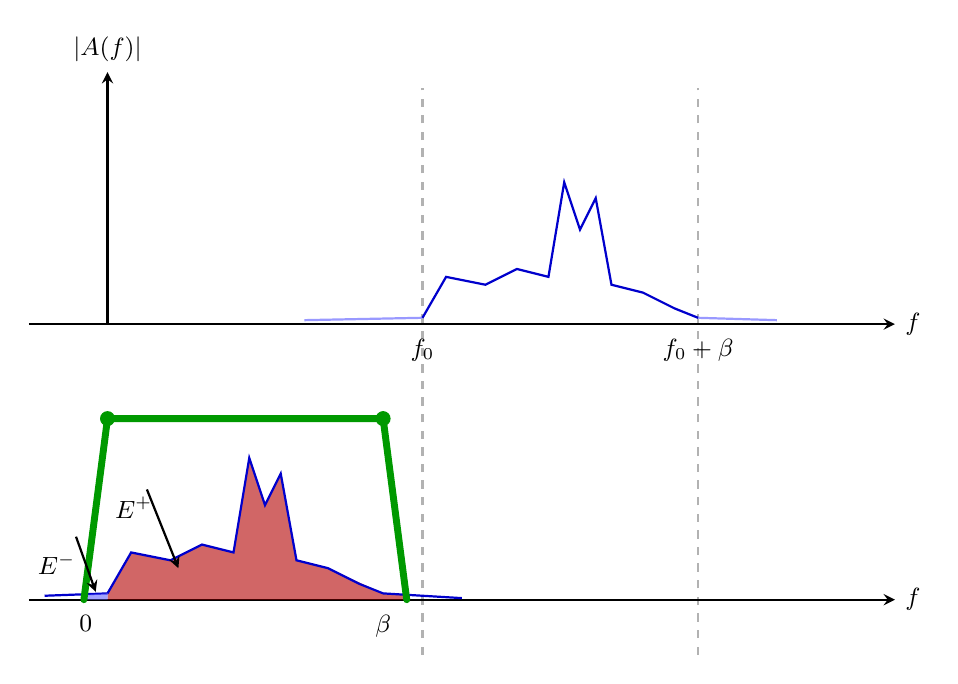
\begin{tikzpicture}[
    font=\small,
    >=stealth
]

    % ==========================================
    % MACRO DE LA SEÑAL (Recibe el desplazamieto en X: #1)
    % ==========================================
    \newcommand{\senoide}[1]{
        \draw[thick, blue!80!black] 
            (#1 + 0.0, 0.08) 
         -- (#1 + 0.3, 0.6) 
         -- (#1 + 0.8, 0.5) 
         -- (#1 + 1.2, 0.7) 
         -- (#1 + 1.6, 0.6) 
         -- (#1 + 1.8, 1.8) 
         -- (#1 + 2.0, 1.2) 
         -- (#1 + 2.2, 1.6) 
         -- (#1 + 2.4, 0.5) 
         -- (#1 + 2.8, 0.4) 
         -- (#1 + 3.2, 0.2) 
         -- (#1 + 3.5, 0.08);
    }

    % ==========================================
    % GRÁFICO SUPERIOR: Banda Pasante (f0 a f0 + Beta)
    % ==========================================
    
    % Eje vertical y horizontal superior
    \draw[thick, ->] (0, 0) -- (0, 3.2) node[above] {\(|A(f)|\)};
    \draw[thick, ->] (-1, 0) -- (10, 0) node[right] {\(f\)};

    % Líneas discontinuas
    \draw[dashed, thick, opacity=0.3] (4, -4.2) -- (4, 3.0);
    \draw[dashed, thick, opacity=0.3] (7.5, -4.2) -- (7.5, 3.0);

    % Etiquetas
    \node[below=2pt] at (4, 0) {\(f_0\)};
    \node[below=2pt] at (7.5, 0) {\(f_0 + \beta\)};

    % Ruido exterior
    \draw[thick, blue!40!white] (2.5, 0.05) -- (4.0, 0.08);
    \draw[thick, blue!40!white] (7.5, 0.08) -- (8.5, 0.05);

    % DIBUJO DE LA SEÑAL SUPERIOR (En f0 = 4.0)
    \senoide{4.0}


    % ==========================================
    % GRÁFICO INFERIOR: Traslación a Banda Base (0 a Beta)
    % ==========================================

    \begin{scope}[yshift=-3.5cm]
        % Eje horizontal inferior
        \draw[thick, ->] (-1, 0) -- (10, 0) node[right] {\(f\)};

        % Referencias
        \node[below left=2pt] at (0, 0) {$0$};
        \node[below=2pt] at (3.5, 0) {\(\beta\)};

        % ÁREA DE ENERGÍA POSITIVA (E+) en Rojo (Alineada con x=0)
        \fill[red!70!black, opacity=0.6] 
            (0.0, 0.0) -- (0.0, 0.1) -- (0.3, 0.6) -- (0.8, 0.5) -- (1.2, 0.7) 
            -- (1.6, 0.6) -- (1.8, 1.8) -- (2.0, 1.2) -- (2.2, 1.6) 
            -- (2.4, 0.5) -- (2.8, 0.4) -- (3.5, 0.08) -- (3.57, 0.07) -- (3.76, 0.06) -- (3.78, 0) -- cycle;

        % DIBUJO DE LA SEÑAL INFERIOR (En f = 0.0)
        \senoide{0.0}

        % Ruido exterior en banda base
        \draw[thick, blue!80!black] (-0.8, 0.05) -- (0.0, 0.08);
        \draw[thick, blue!80!black] (3.5, 0.08) -- (4.5, 0.02);

        % Área aparte de energía negativa (E-)
        \fill[blue!60, opacity=0.6] 
            (-0.3, 0) -- (-0.3, 0.06) -- (0.0, 0.08) -- (0.0, 0.0) -- cycle;

        % Filtro/Máscara Verde en Banda Base
        \draw[line width=2.5pt, green!60!black, line cap=round, line join=round] 
            (-0.3, 0.0) -- (0.0, 2.3) -- (3.5, 2.3) -- (3.8, 0.0);
        
        \filldraw[green!60!black] (0.0, 2.3) circle (2.5pt);
        \filldraw[green!60!black] (3.5, 2.3) circle (2.5pt);

        % Indicadores de anotación
        \draw[->, thick] (-0.4, 0.8) -- (-0.15, 0.1) node[midway, left] {\(E^-\)};
        \draw[->, thick] (0.5, 1.4) -- (0.9, 0.4) node[midway, above left] {\(E^+\)};
    \end{scope}

\end{tikzpicture}%
    }
    \caption{Calibración de \(Q\).}
    \label{fig:cal_Q}
\end{figure}

En la Fig.~\ref{fig:cal_Q} se puede observar que el espectro de interés se encuentra en el intervalo \([f_0,\; f_0+\beta]\), pero se lo debe llevar a banda base \([0,\; \beta]\) aplicando un corrimiento en frecuencia, para luego corregir dicho retardo maximizando la energía positiva en banda base y tomando como energía negativa la correspondiente a las frecuencias negativas, las cuales existen debido al ruido presente.

Esto se logra fácilmente realizando un barrido de posibles retardos y seleccionando aquel que maximice la relación \(\frac{E^{+}}{E^{-}}\).


\subsection{Obtención de indice de refracción}

Al existir una relación lineal entre el tiempo y la frecuencia, es posible determinar la frecuencia $f_{\text{peak}}$ asociada a cada interfaz u objetivo mediante:

\begin{equation}
    f_{\text{peak}} = \frac{\beta}{\tau} t_{\text{peak}} = \frac{\beta}{\tau} \frac{2d_{\text{eq}}}{c}
\end{equation}

Como se observa en la Fig.~\ref{fig:conformal_full_panel}, se obtienen dos picos de frecuencia, $f_1$ y $f_2$. Al calcular el cociente entre ellos:

\begin{equation}
    \frac{f_2}{f_1} = \frac{\frac{\beta}{\tau} \frac{2 d_{\text{eq}, 2}}{c}}{\frac{\beta}{\tau} \frac{2 d_{\text{eq}, 1}}{c}} = \frac{d_{\text{eq}, 1} + n \cdot \text{espesor}}{d_{\text{eq}, 1}}
\end{equation}

donde $d_{\text{eq}, 1}$ es la distancia equivalente a la primera cara de la pastilla y $d_{\text{eq}, 2} = d_{\text{eq}, 1} + n \cdot \text{espesor}$ es la distancia equivalente a la segunda cara. El tiempo que tarda la onda en atravesar el material (ida y vuelta) es $\Delta t = \frac{2 \cdot \text{espesor}}{v_{\text{pastilla}}}$, con la velocidad dentro del medio dada por $v_{\text{pastilla}} = \frac{c}{n}$, siendo $n$ el índice de refracción.

A partir de este cociente, se puede despejar el índice de refracción $n$:

\begin{equation}
    n = \frac{d_{\text{eq}, 1}}{\text{espesor}} \left( \frac{f_2}{f_1} - 1 \right)
    \label{eq:coef_cociente}
\end{equation}

Nótese que esta forma de obtener $n$ depende directamente de qué tan bien esté estimado $d_{\text{eq}, 1}$.

Otra opción para obtener el índice de refracción es mediante la diferencia de frecuencias:

\begin{equation}
    f_2 - f_1 = \frac{\beta}{\tau} \frac{2 d_{\text{eq}, 2}}{c} - \frac{\beta}{\tau} \frac{2 d_{\text{eq}, 1}}{c} = \frac{\beta}{\tau} \frac{2}{c} \left( n \cdot \text{espesor} \right)
\end{equation}

Despejando $n$, se obtiene:

\begin{equation}
    n = \frac{(f_2 - f_1) \cdot c}{2 \left( \frac{\beta}{\tau} \right) \cdot \text{espesor}}
\end{equation}

Nótese que el cálculo del índice de refracción resulta inversamente proporcional al \textit{chirp rate} ($\frac{\beta}{\tau}$) y al espesor de la muestra.

Ademas, estamos asumiento conocido y constante al espesor.


\subsection{Segmentación de material via caracterizacion en espectro}

Al final del pipleline de la figura \ref{fig:calc_peaks} se aplican distintos algortimos de segmentación uno de ellos es el siguiente.

\paragraph{Segementacion no supervisada basada en señales}

Para generar la máscara que va a caracterizar el elemento de estudio, en este caso una pastilla, se debe aplicar una máscara que permita separar la pastilla del fondo.

En sí, es un problema de segmentación al cual se lo ataca con teoría de procesamiento de señales.

\begin{figure}[H]
    \centering
    \resizebox{0.8\textwidth}{!}{%
        
\begin{tikzpicture}[
    font=\small,
    >=stealth,
    block/.style={
        draw, 
        rounded corners=12pt, 
        minimum width=2.4cm, 
        minimum height=2.4cm, 
        align=center, 
        thick
    },
    maskblock/.style={
        draw, 
        rounded corners=12pt, 
        minimum width=2.4cm, 
        minimum height=2.4cm, 
        align=center, 
        thick
    }
]

    % ==========================================
    % 1. BLOQUE DATA Y VECTOR REDUCIDO
    % ==========================================
    
    % Caja principal DATA
    \draw[thick, rounded corners=12pt] (-0.5, -0.4) rectangle (3.0, 3.6);
    \node[above, font=\bfseries] at (1.2, 3.6) {DATA \((N = H \times W)\)};

    % Contenido en columna de DATA
    \node at (1.2, 3.0) {\(\{ f_1, A_1; f_2, A_2 \}_0\)};
    \node at (1.2, 2.3) {\(\{ f_1, A_1; f_2, A_2 \}_1\)};
    \node at (1.2, 1.6) {\(\vdots\)};
    \node at (1.2, 0.9) {\(\{ f_1, A_1; f_2, A_2 \}_j\)};
    \node at (1.2, 0.2) {\(\vdots\)};
    \node at (1.2, -0.2) {\(\{ f_1, A_1; f_2, A_2 \}_N\)};

    % Resaltados verdes verticales
    \fill[green!50!white, opacity=0.4, rounded corners=3pt] (0.55, -0.3) rectangle (1.05, 3.3);
    \fill[green!50!white, opacity=0.4, rounded corners=3pt] (1.80, -0.3) rectangle (2.30, 3.3);

    % Flecha con min(A)
    \draw[thick, ->] (3.1, 1.6) -- node[above, font=\small] {\(\min(A)\)} (3.9, 1.6);

    % Vector de amplitudes reducidas
    \draw[thick, rounded corners=8pt] (4.0, -0.4) rectangle (5.2, 3.6);
    \node at (4.6, 3.0) {\(\{A_1\}_0\)};
    \node at (4.6, 2.3) {\(\{A_2\}_1\)};
    \node at (4.6, 1.6) {\(\vdots\)};
    \node at (4.6, 0.9) {\(\{A_1\}_j\)};
    \node at (4.6, 0.2) {\(\vdots\)};
    \node at (4.6, -0.2) {\(\{A_2\}_N\)};

    % Flecha hacia KNN
    \draw[thick, ->] (5.3, 1.6) -- (6.1, 1.6);


    % ==========================================
    % 2. BLOQUES KNN, ESTIM., FINDPEAKS Y MASK
    % ==========================================

    % Bloque KNN UNSUPERVISED
    \node[block, minimum width=2.4cm] (knn) at (7.35, 1.6) {
        \textbf{KNN}\\[0.1cm]
        \textbf{No}\\[0.05cm]
        \textbf{Supervisado}
    };

    % Bloque ESTIM. DENSIDAD DE DISTANCIAS
    \node[block, minimum width=2.8cm] (dens) at (10.65, 1.6) {
        \textbf{Estim.}\\[0.1cm]
        \textbf{Densidad}\\[0.05cm]
        \textbf{de}\\[0.05cm]
        \textbf{Distancias(A)}
    };

    % Bloque findPeaks
    \node[block, minimum width=3.0cm, minimum height=2.6cm] (peaks) at (14.25, 1.6) {};
    \node[anchor=north, font=\bfseries] at (peaks.north) {findPeaks};

    % Dibujo interno de la señal azul con dos picos
    \draw[thick, ->] (13.05, 0.6) -- (13.05, 2.1) node[left, font=\tiny] {1};
    \draw[thick, ->] (13.05, 0.6) -- (15.35, 0.6);

    % Línea de UMBRAL VERTICAL en el mínimo local entre los dos picos
    \draw[dashed, red!80!black, thick] (14.13, 0.6) -- (14.13, 2.0) node[above, font=\tiny, text=red!80!black] {Umbral};

    \draw[thick, blue!80!black] (13.05, 0.66) 
        to[out=10, in=230] (13.55, 1.05)
        to[out=315, in=179] (14.13, 0.67)
        to[out=358, in=260] (14.75, 1.8)
        to[out=280, in=170] (15.25, 0.65);

    % Bloque Mask
    \node[maskblock, right=1.37cm of peaks] (mask) {};
    \node[anchor=north, font=\bfseries] at (mask.north) {Mask};

    % Coordenada auxiliar para el centro del dibujo de la máscara
    \coordinate (mc) at ([yshift=-0.25cm]mask.center);

    % Dibujo interno en Mask
    \draw[dashed, thick] ([xshift=-0.45cm, yshift=-0.4cm]mc) rectangle ([xshift=0.45cm, yshift=0.4cm]mc);
    \filldraw[fill=green!50!white, draw=black, thick] (mc) circle (0.35cm);
    
    % Onda blanca interna
    \draw[white, line width=1.2pt] ([xshift=-0.2cm]mc) sin ([xshift=-0.1cm, yshift=0.08cm]mc) cos (mc);
    \draw[white, line width=1.2pt] (mc) sin ([xshift=0.1cm, yshift=-0.08cm]mc) cos ([xshift=0.2cm]mc);

    % Conexiones principales
    \draw[thick, ->] (knn) -- (dens);
    \draw[thick, ->] (dens) -- (peaks);

    % Salidas de findPeaks hacia Mask
    \draw[thick, ->] ([yshift=0.3cm]peaks.east) -- node[above, font=\tiny] {\([A_i \in \mathcal{A}]\)} ([yshift=0.3cm]mask.west);

\end{tikzpicture}
%
    }
    \caption{Algoritmo de generación de máscara con KNN no supervisado.}
    \label{fig:maskv0}
\end{figure}

En la Fig.~\ref{fig:maskv0}, de las señales se obtienen los dos picos máximos, de los cuales solo nos interesan las dos amplitudes y quedarnos con el pico máximo $A_i$, el cual se presume que corresponde a \(f_1\), la frecuencia respectiva al primer rebote.

Luego, se procede a aplicar KNN no supervisado, el cual nos devuelve las distancias (en amplitud) de cada punto respecto a las demás. Con ello se puede calcular una densidad de distancias y así poder trazar un umbral para separar al primer pico que del segundo pico, para mediante eso poder clasificar y así generar la máscara $\mathcal{A}$ tal que es el conjunto de pixeles que conforman la pastilla,quien no pertenecezca a dicho conjunto será fondo..



\paragraph{Segmentación no supervisada basada en imágenes}

La siguiente solución está basada en la segmentación, en donde las entradas y la salida son imágenes.

La imagen de entrada se obtiene a partir de calcular, para cada píxel, el respectivo coeficiente de refracción, como se ve por ejemplo en la ecuación \eqref{eq:coef_cociente}.

El problema con esto viene dado por la simple estimación de picos mediante \textit{findPeaks}; con ello se obtienen coeficientes \(n\) demasiado ruidosos. Este escenario presenta zonas en donde el objeto está bien definido y también lo está el fondo, pero en los bordes o fronteras entre las dos clases hay demasiado ruido para distinguir el objeto del fondo. Por ello, se opta por \textbf{segmentar texturas}, para lo cual se propone el siguiente pipeline:

\begin{figure}[H]
    \centering
    \resizebox{0.8\textwidth}{!}{        \begin{tikzpicture}[
    font=\small,
    >=stealth,
    block/.style={
        draw, 
        rounded corners=12pt, 
        minimum width=2.4cm, 
        minimum height=2.4cm, 
        align=center, 
        thick
    },
    maskblock/.style={
        draw, 
        rounded corners=12pt, 
        minimum width=2.4cm, 
        minimum height=2.4cm, 
        align=center, 
        thick
    }
]

    % ==========================================
    % 1. ENTRADA: IMAGEN RUIDOSA DE LA PASTILLA
    % ==========================================
    
    % Caja Imagen I (Ruidosa)
    \draw[thick, rounded corners=12pt] (-0.5, 0.25) rectangle (2.25, 2.93);
    \node[above, font=\bfseries] at (0.85, 3.6) {Imagen \(I\) (Ruidosa)};
    
    % Ilustración de la pastilla con ruido interno
    \draw[thick, fill=gray!20, dashed] (0.85, 1.6) circle (0.8cm);
    \node[font=\tiny, align=center] at (0.85, 1.6) {Pastilla\\+ Ruido};
    \node[font=\tiny, gray] at (0, 2.73) {\(\cdot \cdot \times\)};
    \node[font=\tiny, gray] at (1.73, 0.72) {\(\times \cdot \cdot\)};

    % Flecha hacia Banco de Gabor / Matriz X
    \draw[thick, ->] (2.3, 1.6) -- node[above, font=\tiny] {16 Filtros} node[below, font=\tiny] {Gabor} (3.2, 1.6);


    % ==========================================
    % 2. MATRIZ X Y K-MEANS (TEXTONES)
    % ==========================================

    % Matriz X de Respuestas
    \draw[thick, rounded corners=8pt] (3.3, -0.4) rectangle (4.9, 3.6);
    \node[above, font=\bfseries] at (4.1, 3.6) {Matriz \(X\)};
    
    \node at (4.1, 3.0) {\tiny \([r_1 \dots r_{16}]_0\)};
    \node at (4.1, 2.3) {\tiny \([r_1 \dots r_{16}]_1\)};
    \node at (4.1, 1.6) {\(\vdots\)};
    \node at (4.1, 0.9) {\tiny \([r_1 \dots r_{16}]_j\)};
    \node at (4.1, 0.2) {\(\vdots\)};
    \node at (4.1, -0.2) {\tiny \([r_1 \dots r_{16}]_N\)};

    % Flecha hacia KMeans
    \draw[thick, ->] (4.9, 1.6) -- (5.7, 1.6);

    % Bloque KMeans Textons
    \node[block, minimum width=2.4cm] (km1) at (6.9, 1.6) {
        \textbf{K-Means}\\[0.1cm]
        \tiny Textones\\
        \tiny (\(K_1 = 10\))
    };

    % Flecha a Mapa de Textones
    \draw[thick, ->] (km1) -- (8.46, 1.6);


    % ==========================================
    % 3. MAPA DE TEXTONES Y HISTOGRAMAS
    % ==========================================

    % Mapa de Textones (H x W)
    \draw[thick, rounded corners=8pt] (8.5, -0.4) rectangle (10.1, 3.6);
    \node[anchor=north, font=\bfseries, align=center] at (9.3, 3.5) {\footnotesize Texton\\[-0.05cm]\footnotesize Map};
    
    % Ventana 21x21 sobre el Texton Map
    \draw[dashed, red!80!black, thick] (8.8, 1.1) rectangle (9.8, 2.1);
    \node[font=\tiny, text=red!80!black] at (9.3, 0.8) {Ventana \(21\times21\)};

    % Flecha hacia Histograma Local
    \draw[thick, ->] (10.2, 1.6) -- (11.0, 1.6);

    % Matriz de Histogramas Locales
    \draw[thick, rounded corners=8pt] (11.1, -0.4) rectangle (12.8, 3.6);
    \node[anchor=north, font=\bfseries, align=center] at (11.95, 3.5) {\footnotesize Matriz\\[-0.05cm]\footnotesize Hist.};
    
    \node at (11.95, 2.4) {\tiny \(\mathbf{h}_0 \in \mathbb{R}^{10}\)};
    \node at (11.95, 1.8) {\tiny \(\mathbf{h}_1 \in \mathbb{R}^{10}\)};
    \node at (11.95, 1.3) {\(\vdots\)};
    \node at (11.95, 0.75) {\tiny \(\mathbf{h}_j \in \mathbb{R}^{10}\)};
    \node at (11.95, 0.15) {\(\vdots\)};
    \node at (11.95, -0.15) {\tiny \(\mathbf{h}_N \in \mathbb{R}^{10}\)};

    % Flecha hacia GMM
    \draw[thick, ->] (12.9, 1.6) -- (13.7, 1.6);


    % ==========================================
    % 4. GMM Y SALIDA MÁSCARA (TU BLOQUE ORIGINAL)
    % ==========================================

    % Bloque GMM
    \node[block, minimum width=2.4cm] (gmm) at (14.9, 1.6) {
        \textbf{GMM}\\[0.1cm]
        \tiny Regiones\\
        \tiny (\(K_2 = 10\))
    };

    % Bloque Mask (Misma construcción e identidad visual exacta que el anterior)
    \node[maskblock, right=1.02cm of gmm, minimum width=78.4613287pt, minimum height=79.6677171pt] (mask) {};
    \node[anchor=north, font=\bfseries] at (mask.north) {Mask};

    % Coordenada auxiliar para el centro del dibujo de la máscara
    \coordinate (mc) at ([yshift=-0.25cm]mask.center);

    % Dibujo interno en Mask
    \draw[dashed, thick] ([xshift=-0.45cm, yshift=-0.4cm]mc) rectangle ([xshift=0.45cm, yshift=0.4cm]mc);
    \filldraw[fill=green!50!white, draw=black, thick] (mc) circle (0.9cm);
    
    % Onda blanca interna
    \draw[white, line width=1.2pt] ([xshift=-0.2cm]mc) sin ([xshift=-0.1cm, yshift=0.08cm]mc) cos (mc);
    \draw[white, line width=1.2pt] (mc) sin ([xshift=0.1cm, yshift=-0.08cm]mc) cos ([xshift=0.2cm]mc);

    % Conexión final desde GMM hacia Mask
    \draw[thick, ->] (gmm) -- (mask.west);

\end{tikzpicture}}
    \caption{Segmentación mediante filtros de Gabor....}
    \label{fig:maskv1_gabor}
\end{figure}

Como se ve en la Fig.~\ref{fig:maskv1_gabor}, la imagen pasa por dos agrupamientos distintos:

\begin{itemize}
    \item Se le aplican \(M\) filtros de Gabor a la imagen, lo que genera \(M\) nuevas características (\textit{features}) por cada píxel.
    \item Luego se realiza un agrupamiento con algún algoritmo de \textit{clustering}, por ejemplo K-Means, recuperando así la dimensión original pero con los píxeles agrupados.
    \item A este nuevo espacio se lo conoce como mapa de \textit{textones}, al cual se le calcula un histograma local tomado a través de una ventana deslizante, obteniendo así un nuevo espacio de histogramas.
    \item Finalmente, en este nuevo espacio se realiza un segundo agrupamiento con las clases que uno espera obtener; en este caso se utilizó GMM.
\end{itemize}
